\documentclass[12pt]{article}
\usepackage{geometry} % see geometry.pdf on how to lay out the page. There's lots.
\geometry{a4paper} % or letter or a5paper or ... etc
\usepackage{graphicx}
\setlength{\parindent}{0.0in}
\setlength{\parskip}{0.1in}

% \geometry{landscape} % rotated page geometry

% See the ``Article customise'' template for come common customisations

\title{SteelSeries GoLisp \\ {\small\it An embeddable scripting system for Go}}
\author{Dave Astels \\ SteelSeries NA Corp.}

\begin{document}

\maketitle

\section{Overview}

GoLisp is a simple Lisp language and runtime implimented in Google's
Go programming language. It's main purpose is integration into a Go
application to provide runtime extension and scripting. The core of a
basic Lisp in provided, but with limited special forms and primitive
functions. More of these will be added as required without having to
modify the GoLisp core. Also, a REPL is provided and GoLisp can be
used as-is to write and evaluage code.

GoLisp is a lexically scoped Lisp-1:

\begin{description}
\item[Lexically scoped:] The scope of definitions are determined by
  where they are made in the lexical structure of the code. Each
  function, \verb|let|, and \verb|do| creates a new lexical scope. From~\cite{Gabriel:1988:ETI}:

  \begin{quotation}
    Here references to the established entity can occur only within
    certain program portions that are lexically (that is, textually)
    contained within the establishing construct. Typically the
    construct will have a part designated the body, and the scope of
    all entities established will be (or include) the body.
  \end{quotation}

\item[Lisp-1:] A Lisp where functions and variables share a single
  namespace. This differs from a Lisp-2 in which functions and
  variables have separate namespaces.
\end{description}

The GoLisp REPL supports \verb|readline| and so provides history and
command editing. History is local to the directory from which you
execute GoLisp.

\section{Data types}

\begin{description}

\item[Cons Cells] are the central data type in classic Lisp used both
  as dotted pairs \verb|(a .  b)| and general lists \verb|(a b)|. For
  an overview of cons cells and how to use them
  see~\cite{Abelson85Structure}, \cite{Steele:1984:CLL}, or
  \verb|http://cs.gmu.edu/~sean/lisp/cons/|.

\item[Symbols] are simple identifiers, e.g. \verb|function-name|.
Symbols follow the follow 2 simple rules:

\begin{itemize}
\item starts with a letter, and
\item contains alphanumeric, \verb|-|, \verb|_|, \verb|?|, \verb|!|, and \verb|*|.
\end{itemize}

Typically, \verb|-| is used to seperate words in a symbol, \verb|_| is
used in special symbols (such as system use) to separate words and as
a prefix and suffix. The characters \verb|?|, \verb|!|, and \verb|*|
are typically used as the final character of a function name to
denote:

\begin{description}
\item [?] a predicate, e.g. \verb|nil?|
\item [!] a mutating function (changes the argument rather than
  returning a modified copy), e.g. \verb|set-car!|
\item [*] a varient of the primary function, e.g. \verb|flatten|
  (which does a one level flattening of a list) and \verb|flatten*|
  (which is a recursive \verb|flatten|)
\end{description}

Some builtin function names violate these rules (e.g. arithmetic and
relative functions). You can't create symbols like this without
adding support for them to the tokenizer and parser.

\item[Strings] are any sequence of characters other than \verb|"|
enclosed by a pair of \verb|"|, e.g. \verb|"string"|.

\item[Integers] are non-negative integers internally represented as \verb|uint32|. Both decimal and hexidecimal formats are supported. E.g.
  \verb|26|, \verb|0x1a|, \verb|0x1A|.

\item[Floats] are Go \verb|float32| numbers. Accordingly they are
  signed. All arithmetic functions with the exception of modulus work
  as expected for both numbers and floats. Numbers are coerced to
  floats as required, specifically if any arguments are float, all are
  converted to float and the result will be a float.

\item[Booleans] represent true and false. \verb|nil|, \verb|()|, and
\verb|false| are all logically false, everything else is logically true.
Boolean literals are \verb|#t| and \verb|#f| for true and false,
respectively.

\item[Functions] are user defined procedures. They are covered in
detail later.

\item[Objects] allow you to encapsulate a Go object (struct) in a Lisp
  data object. There is no way to do this from Lisp itself, but is
  useful when writing primitive functions (see below).

\item[Bytearrays] are simply objects that encapsulate \verb|[]byte|
  objects. The difference is that there is syntactic support for them.
  Use square braces surrounding a list of numbers between 0 and 255.
  For example: \verb|[1 2 3 4 5]|. That format will parse to an
  \verb|object| containing a the Go bytearray (i.e. \verb|[]byte|).
  Bytearrays evaluate to themselves.

\item[Primitives] are just as they are in Lisp or Smalltalk: functions
  written in Go and exposed as functions in Lisp. The combination of
  primitives and objects allow you to integrate with the underlying Go
  program.
\end{description}

\section{Builtin functions}

\subsection{Arithmetic}

\noindent{\bf\large\verb|(+ <number>...)|}

Adds a series of numbers, e.g.

\begin{verbatim}
    (+ 4) ==> 4
    (+ 4 2) ==> 6
    (+ 4 2 7) ==> 13
    (+ 1.2 2.3) ==> 3.5
    (+ -1.2 2.3) ==> 1.0999999
\end{verbatim}

\noindent{\bf\large\verb|(- <number>...)|}

Sequentially subtracts a sequence of numbers. Negative results become
0 for integers, while negative results are supported for float subtraction. E.g.

\begin{verbatim}
    (- 10 3) ==> 7
    (- 10 3 4) ==> 3
    (- 10 3 4 5) ==> 0
    (- 2.3 1.2) ==> 1.0999999
    (- 1.2 2.3) ==> -1.0999999
\end{verbatim}

\noindent{\bf\large\verb|(* <number>...)|}

Multiplies a series of numbers, e.g.

\begin{verbatim}
    (* 4) ==> 4
    (* 4 2) ==> 8
    (* 4 2 7) ==> 56
    (* 1.2 2.3) ==> 2.76
\end{verbatim}

\noindent{\bf\large\verb|(/ <number>...)|}

Sequentially divides a sequence of numbers. E.g.

\begin{verbatim}
    (/ 30 2) ==> 15
    (/ 30 2 3 ) ==> 5
    (/ 30 4) ==> 7
    (/ 30.0 4) ==> 7.5
\end{verbatim}

\noindent{\bf\large\verb|(% <number> <number>)|}

Returns the remainder of dividion. NOTE: modulus only works for
integers. E.g.

\begin{verbatim}
    (% 4 2) ==> 0
    (% 4 3) ==> 1
\end{verbatim}

\subsection{Conversions}

\noindent{\bf\large\verb|(integer <number>)|}

Returns the integer value of \verb|<number>|. If it is an integer, it
is simply returned. However, if it is a float the integer part is
returned. Note that this is implemented in go by casting the
\verb|float32| to a \verb|uint32| so converting negative floats gives
a large integer.

\begin{verbatim}
    (integer 5) ==> 5
    (integer 5.2) ==> 5
    (integer 5.8) ==> 5
    (integer -1.0) ==> 4294967295
\end{verbatim}

\noindent{\bf\large\verb|(float <number>)|}

Returns the float value of \verb|<number>|. If it is a float, it
is simply returned. However, if it is an integer the coresponding float is
returned.

\begin{verbatim}
    (float 5) ==> 5.0
\end{verbatim}

Note that converting a float to a string for printing using the format
\verb|%g| to use the minimum number of characters so \verb|5.0| will
actually print as \verb|5|.

\subsection{Comparisons}

All comparison operations work with floating point numbers as well.

\noindent{\bf\large\verb|(< <number> <number>)|}

Returns whether the first argument is less than the second argument.

\begin{verbatim}
    (< 1 2) ==> #t
    (< 2 1) ==> #f
    (< 2 2) ==> #f
\end{verbatim}

\noindent{\bf\large\verb|(> <number> <number>)|}

Returns whether the first argument is greater than the second argument.

\begin{verbatim}
    (> 1 2) ==> #f
    (> 2 1) ==> #t
    (> 2 2) ==> #f
\end{verbatim}

\noindent{\bf\large\verb|(== <number> <number>)|}

Returns whether the first argument is equal to the second argument.

\begin{verbatim}
    (== 1 2) ==> #f
    (== 1 1) ==> #t
\end{verbatim}

\noindent{\bf\large\verb|(!= <number> <number>)|}

Returns whether the first argument is not equal to the second argument.

\begin{verbatim}
    (!= 1 2) ==> #t
    (!= 1 1) ==> #f
\end{verbatim}

\noindent{\bf\large\verb|(<= <number> <number>)|}

Returns whether the first argument is less than or equal to the second
argument.

\begin{verbatim}
    (<= 1 2) ==> #t
    (<= 2 1) ==> #f
    (<= 2 2) ==> #t
\end{verbatim}

\noindent{\bf\large\verb|(>= <number> <number>)|}

Returns whether the first argument is greater than or equal to the
second argument.

\begin{verbatim}
    (>= 1 2) ==> #f
    (>= 2 1) ==> #t
    (>= 2 2) ==> #t
\end{verbatim}

\noindent{\bf\large\verb|(odd? <number>)|}

Returns whether the argument is odd.

\begin{verbatim}
    (odd? 2) ==> #f
    (odd? 5) ==> #t
\end{verbatim}

\noindent{\bf\large\verb|(even? <number>)|}

Returns whether the argument is even.

\begin{verbatim}
    (even? 2) ==> #t
    (even? 5) ==> #f
\end{verbatim}

\noindent{\bf\large\verb|(random-byte)|}

Returns a psuedo-random unsigned integer between 0 and 255, inclusive..

\begin{verbatim}
    (random-byte) ==> 13
    (random-byte) ==> 207
\end{verbatim}

\subsection{Logical}

\noindent{\bf\large\verb|(! <arg>)|}
\noindent{\bf\large\verb|(not <arg>)|}

Returns whether the boolean negation of the argument.

\begin{verbatim}
    (! #t) ==> #f
    (! #f) ==> #t
\end{verbatim}

\noindent{\bf\large\verb|(and <arg>)|}

Computes a logical and of the arguments (which are evaluated first),
with shortcutting. I.e. each argument is evaluated in order until one
evaluates to false or the end of the list is reached. If all evaluate
to true the result of the \verb|and| is true, otherwise it is false.
If an argument evaluates to false, subsequent arguments are not
evaluated. \verb|and| with no arguments evaluates to true.

\begin{verbatim}

\end{verbatim}

\noindent{\bf\large\verb|(or <arg>)|}

Computes a logical or of the arguments (which are evaluated first),
with shortcutting. I.e. each argument is evaluated in order until one
evaluates to true or the end of the list is reached. If all evaluate
to false the result of the \verb|or| is false, otherwise it is true.
If an argument evaluates to true, subsequent arguments are not
evaluated. \verb|or| with no arguments evaluates to false.

\begin{verbatim}

\end{verbatim}

\subsection{Lists}

\noindent{\bf\large\verb|(list <arg>...)|}

Creates a list out of a sequence of values.

\begin{verbatim}
  (list 1 2 3) ==> (1 2 3)
  (list (+ 1 1) (+ 2 2) (+ 3 3)) ==> (2 4 6)
\end{verbatim}

\noindent{\bf\large\verb|(append <list> <sexpr>)|}

Append the result of evaluating \verb|<sexpr>| to \verb|<lsit>|. This
makes a copy of \verb|<list>|, appends to it, and returns the copy
(which now contains the appened item).

\noindent{\bf\large\verb|(append! <list> <sexpr>)|}

Append the result of evaluating \verb|<sexpr>| to \verb|<lsit>|. This
appends to the list provided, and returns it. The side effect
(indicated by the \verb|!|) is that the original list is modified,
unlike using \verb|append|..
For example:

\begin{verbatim}
  (define a '(1 2 3))
  (append a '(4 5 6)) => (1 2 3 4 5 6)
  a => (1 2 3)

  (append! a '(4 5 6)) => (1 2 3 4 5 6)
  a => (1 2 3 4 5 6)
\end{verbatim}

\noindent{\bf\large\verb|(interval <lo> <hi>)|}

Creates a list of numbers from \verb|<lo>| to \verb|<hi>|, inclusive.

\begin{verbatim}
  (interval 1 5) ==> (1 2 3 4 5)
\end{verbatim}

\noindent{\bf\large\verb|(car <list>)|}\\
\noindent{\bf\large\verb|(first <list>)|}

Returns the first item in the list, i.e. the car pointer of the first
conscell in the chain referenced by \verb|<list>|.

\begin{verbatim}
  (car nil) ==> nil
  (car '(a)) ==> a
  (car '(a b c)) ==> a
  (car (list (+ 1 1) (+ 2 2))) ==> 2
\end{verbatim}

\noindent{\bf\large\verb|(cdr <list>)|}\\
\noindent{\bf\large\verb|(rest <list>)|}

Returns the rest of the list, i.e. the cdr pointer of the first
conscell in the chain referenced by \verb|<list>|. \verb|rest| is provided as an alias.

\begin{verbatim}
  (cdr nil) ==> nil
  (cdr '(a)) ==> nil
  (cdr '(a b c)) ==> (b c)
  (cdr (list (+ 1 1) (+ 2 2))) ==> (2)
\end{verbatim}

The above \verb|car| and \verb|cdr| functions are the fundamental list
decomposition operations. There are more that are based on these two.
First there are a series of functions explicitly using \verb|car| and
\verb|cdr| such as \verb|caddr| which is equivalent to
\verb|(car (cdr (cdr <list>)))|. Up to \verb|cddddr| is supported.

\begin{verbatim}
  (caddr '(1 2 3 4 5)) ==> 3
  (cdddr '(1 2 3 4 5)) ==> (4 5)
\end{verbatim}

\noindent{\bf\large\verb|(first <list>)|}\\
\noindent{\bf\large\verb|(second <list>)|}\\
\noindent{\bf\large\verb|(third <list>)|}\\
\noindent{\bf\large\verb|(fourth <list>)|}\\
\noindent{\bf\large\verb|(fifth <list>)|}

These do exactly what you'd think: return the first, second, etc item
from the list.

\noindent{\bf\large\verb|(nth <list> n)|}

Returns the nth element, starting with 1.

\begin{verbatim}
  (nth '(1 2 3 4) 3) ==> 3
\end{verbatim}

\subsection{Association lists}

Association lists (aka a-lists) are a classic Lisp way to handle associating a value
with a key. Implimentation is a list of dotted pairs: the \verb|car|
is the key, and the \verb|cdr| is the value.

\noindent{\bf\large\verb|(acons <key> <value> [<a-list>])|}

This returns the result of adding a pair \verb|(<key> . <value>)| to
<a-list>. \verb|<key>|, \verb|<value>|, and \verb|<a-list>| are
evaluated. If \verb|<a-list>| is ommitted, it defaults to \verb|nil|.

\begin{verbatim}
  (acons 'a 1) ==> ((a . 1))
  (acons 'a 1 '((b . 2) (c . 3))) ==> ((a . 1) (b . 2) (c . 3)))
\end{verbatim}

\noindent{\bf\large\verb|(pairlis <keys> <values>)|}
\noindent{\bf\large\verb|(pairlis <keys> <values> <a-list>)|}

Creates an a-list from lists of keys and values. A third argument can
be provided which is an exicting a-list that the new pairs will be
added to.

\begin{verbatim}
  (pairlis '(a b) '(1 2)) ==> ((b.2) (a.1)))
  (pairlis '(a b) '(1 2) '((c.3) (d.4))) ==> ((b.2) (a.1) (c.3) (d.4))))
\end{verbatim}

Now that we have a way to create a-lists, we have a couple functions
to get data out of them.\\

\noindent{\bf\large\verb|(assoc <key> <a-list>)|}

Return the pair from \verb|<a-list>| whose \verb|car| is equal to
\verb|<key>|. The empty pair is returned is \verb|<key>| isn't found.

\begin{verbatim}
  (assoc 'a '((a.1) (b.2) (c.3))) ==> (a.1)
  (assoc 'c '((a.1) (b.2))) ==> ()
\end{verbatim}

\noindent{\bf\large\verb|(rassoc <value> <a-list>)|}

Return the pair from \verb|<a-list>| whose \verb|cdr| is equal to
\verb|<value>|. The empty pair is returned is \verb|<value>| isn't found.

\begin{verbatim}
  (rassoc '1 '((a.1) (b.2) (c.3))) ==> (a.1)
  (rassoc '3 '((a.1) (b.2))) ==> ()
\end{verbatim}

\section{Bytearrays}

\noindent{\bf\large\verb|(list-to-bytearray <list of bytes>)|}

The list must be comprised of numbers between 0 and 255, inclusive.
The result is an \verb|object| containing a \verb|[]byte|.

\begin{verbatim}
  (list-to-bytearray '(1 2 3 4)) => [1 2 3 4]
\end{verbatim}

\noindent{\bf\large\verb|(bytearray-to-list <bytearray>)|}

This is the opposite of the previous function. The result is a list
containing the numbers in the bytearray.

\begin{verbatim}
  (bytearray-to-list [1 2 3 4]) => (1 2 3 4)
\end{verbatim}

\noindent{\bf\large\verb|(replace-byte <bytearray> <index> <value>)|}

Make a copy of \verb|<bytearray>| and replaces the byte at
\verb|<index>| with \verb|<value>|. The new bytearray with the
replaced byte is returned.
\verb|<index>| must be a valid index into the byte array (zero based), and
\verb|<value>| must be a valid byte value, i.e. between 0 and 255, inclusive.

\begin{verbatim}
  (define a [1 2 3 4])    => [1 2 3 4]
  (replace-byte a 2 100)  => [1 2 100 4]
  a                       => [1 2 3 4]
\end{verbatim}

\noindent{\bf\large\verb|(replace-byte! <bytearray> <index> <value>)|}

Replaces the byte at \verb|<index>| with \verb|<value>|.
\verb|<index>| must be a valid index into the byte array (zero based), and
\verb|<value>| must be a valid byte value, i.e. between 0 and 255,
inclusive. The original byte array is modified and the returned
bytearray object is the one that is passed to the function.

\begin{verbatim}
  (define a [1 2 3 4])    => [1 2 3 4]
  (replace-byte! a 2 100) => [1 2 100 4]
  a                       => [1 2 100 4]

\end{verbatim}

\noindent{\bf\large\verb|(extract-byte <bytearray> <index>)|}

Fetch and return the byte at \verb|<index>|.
\verb|<index>| must be a valid index into the byte array (zero based).

\begin{verbatim}
  (extract-byte [1 2 3 4] 2) => 3
\end{verbatim}

\noindent{\bf\large\verb|(append-bytes <bytearray> <byte>...)|}\\
\noindent{\bf\large\verb|(append-bytes <bytearray> <list of bytes>)|}\\
\noindent{\bf\large\verb|(append-bytes <bytearray> <bytearray>)|}

Appends the rest of the arguments to a copy of the bytearray that is the first
arg. The copy is returned. Things that can be appended are:
\begin{itemize}
\item A single byte
\item A sequence of bytes (as a sequence of separate arguments)
\item A list of bytes
\item A bytearray object
\item Code that evaluates to a byte, list of bytes, or bytearray.
\end{itemize}

\begin{verbatim}
  (append-bytes [1 2 3] 4)            => [1 2 3 4]
  (append-bytes [1 2 3] 4 5 6)        => [1 2 3 4 5 6]
  (append-bytes [1 2 3] '(4 5 6))     => [1 2 3 4 5 6]
  (append-bytes [1 2 3] [4 5 6])      => [1 2 3 4 5 6]
  (append-bytes [1 2 3] (list 4 5 6)) => [1 2 3 4 5 6]
\end{verbatim}

\noindent{\bf\large\verb|(append-bytes! <bytearray> <byte>...)|}\\
\noindent{\bf\large\verb|(append-bytes! <bytearray> <list of bytes>)|}\\
\noindent{\bf\large\verb|(append-bytes! <bytearray> <bytearray>)|}

As with \verb|append-bytes|, but modifies and returns the bytearray
that is passed in rather than making a copy.

\begin{verbatim}
  (define a [1 2 3])  => [1 2 3]
  (append-bytes a 4)  => [1 2 3 4]
  a                   => [1 2 3]
  (append-bytes! a 4) => [1 2 3 4]
  a                   => [1 2 3 4]
\end{verbatim}

\section{Utility}

\noindent{\bf\large\verb|(sleep <millis>)|}

Sleep for \verb|<millis>| milliseconds.

\begin{verbatim}
  (sleep 1000)  ;; resumes execution 1 second later
\end{verbatim}

\noindent{\bf\large\verb|(write-line <sexpr>)|}

Writes the string form of \verb|<sexpr>|.

\begin{verbatim}
  (write-line "Hello, world.")  ;; Hello, world. is sent to the console.
\end{verbatim}

\noindent{\bf\large\verb|(str <sexpr>...)|}

Creates a string from contatenating the string forms of all the \verb|<sexpr>|s.

\begin{verbatim}
  (str 1 "." 2) ==> "1.2"
\end{verbatim}

\noindent{\bf\large\verb|(copy <sexpr>)|}

Make a copy of the result of evaluating \verb|<sexpr>|, IFF it's
mutable. This is limited to lists and association lists. All other
values are immutable. Copying an immutable item will return the item,
whereas copying a list or assocaition list will make a deep copy of
the structure, and retuen it.

\section{Special forms}

\noindent{\bf\large\verb|(quote <expr>)|}

Surpresses evaluation of the expression.

\begin{verbatim}
     (quote (+ 1 2)) ==> (+ 1 2)
\end{verbatim}

There is a shortcut for quote that uses the single quote:

\begin{verbatim}
    '(+ 1 2) ==> (+ 1 2)
\end{verbatim}

\noindent{\bf\large\verb|(cond (<predicate> <sexpr>...)...)|}

Each predicate is evaluated in order until one results in true value.
The expressions associated with this predicate are then evaluated in order,
and the result of the \verb|cond| is the result of the last
evaluation. If all predicates evaluate to false values, the value of
cond in indeterminate. If, however, the final predicate is the symbol
\verb|else| the expressions associated with it are evaluated, and the
value of \verb|cond| is the value of the last evaluation.

\begin{verbatim}
  (cond ((> 3 2) 'greater)
        ((< 3 2) 'less)) ==> greater

  (cond ((> 3 3) 'greater)
        ((< 3 3) 'less)
        (else 'equal)) ==> equal
\end{verbatim}

\noindent{\bf\large\verb|(case <target sexpr> (<value> <sexpr>...)... [else <sexpr>...]|}

\verb|case| chooses code to evaluate based on the value of the target
sexpr. Any number of expressions can be associated with each target value.

\begin{verbatim}
(define (test-func x)
  (case x
    (0 "zero")
    (1 "one")
    (2 "two")
    (3 "three")
    (else "unknown")))

(test-func 0) ==> "zero"
(test-func 1) ==> "one"
(test-func 2) ==> "two"
(test-func 3) ==> "three"
(test-func 5) ==> "unknown"
\end{verbatim}

\noindent{\bf\large\verb|(if <condition> <true clause>)|}

This is a special case of \verb|cond| that is more familiar to
programmers used to Algol style languages. \verb|if| has two forms,
one that conditionally evaluates a single sexpr (see below about
\verb|begin| which provides a way to use multiple sexprs in this context).

Iff the condition evaluates to logically true, the true clause is
evaluated and the result is the result of the if form, otherwise nil
is the result of the if form.

\begin{verbatim}
    (if (< 1 2)
        "less") ==> "less"
    (if (< 2 2)
        "less") ==> nil
\end{verbatim}

\noindent{\bf\large\verb|(if <condition> <true clause> <else clause>)|}

If the condition evaluates to logically true, the true clause is
evaluated and the result is the result of the if form, otherwise the
else clause is evaluated and is the result of the if form.

\begin{verbatim}
    (if (< 1 2)
        "less"
        "not less") ==> "less"
    (if (< 2 2)
        "less"
        "not less") ==> "not less"
\end{verbatim}

\noindent{\bf\large\verb|(lambda (<param>...) <expr>...)|}

Creates an anonymous function. This can then be used in a function call.

\begin{verbatim}
    ((lambda (x)
       (+ x x))
     5) ==> 10
\end{verbatim}

\verb|lambda| creates a local environment at the point of it's
evaluation. This environment is attached to the resulting function,
and any binding or symbol lookup starts in this local environment. For
example, consider the following code (from~\cite{Abelson85Structure}, \S~3.2.2):

\begin{verbatim}
  (define (square x)
     (* x x))

   (define (sum-of-squares x y)
     (+ (square x) (square y)))

   (define (f a)
     (sum-of-squares (+ a 1) (* a 2)))
\end{verbatim}

Each of the three functions have their own associated definition
environment pointer that points back to the global environment.

When a fucntion is executed, the implicit \verb|lambda| creates a new
envroment frame for the evaluation that (in this case) points back to
the global environment. This scoping approach is what is described in
\S~3 of \cite{Abelson85Structure}.

\begin{figure}[htbp] %  figure placement: here, top, bottom, or page
   \centering
   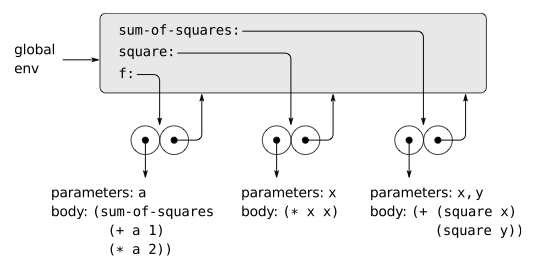
\includegraphics[width=5in]{function_declarations.png}
\caption{Procedure objects in the global frame.}
\label{fig:funcdefs}
\end{figure}

\begin{figure}[htbp] %  figure placement: here, top, bottom, or page
   \centering
   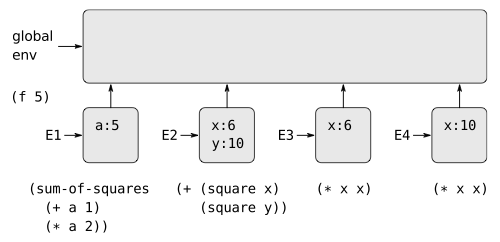
\includegraphics[width=5in]{function_invocations.png}
\caption[Invocation Environments]{Environments created by evaluating
  {\tt (f 5)} using the procedures in Figure~\ref{fig:funcdefs}.}
\label{fig:funcinvocations}
\end{figure}


\noindent{\bf\large\verb|(define <symbol> <value>)|}

Evaluates the value expression and binds it to the symbol, returning
the value.

\begin{verbatim}
    (define x (+ 2 3)) ==> 5
    x ==> 5
\end{verbatim}

Functions can be named (i.e. bound to a symbol) and later referred to
by using define:

\begin{verbatim}
  (define foo (lambda (x)
                (+ x x)))
  (foo 5) ==> 10
\end{verbatim}


\noindent{\bf\large\verb|(define (<symbol> <param>...) <body>)|}

A syntacticly cleaner way to create a named function:

\verb|<symbol>| specifies the name (how you reference the function)

\verb|<param>...| parameters of the function, these are bound to the
respective arguments when the function is called.

\verb|<body>| the sequence of expressions that are evaluated in order
when the function is called. The final evaluation result becomes the
value of evaluation of the function.

\begin{verbatim}
    (define (double x)
       (+ x x))
    (double 5) ==> 10
\end{verbatim}

\noindent{\bf\large\verb|(apply <function> <sexpr>...)|}

Apply the function that results from evaluating \verb|<function| to
the argument list resulting from evaluating each \verb|<sexpr>|.

\noindent{\bf\large\verb|(set! <name> <new-value>)|}

The way to assign (i.e. rebind) a symbol. \verb|name| is the symbol to
be rebound. The \verb|new-value| sexpr is evaluated to arrive at the
new value to be bound to. Use of \verb|set!| is frowned upon, and
should not be used without thought.  See Chapter 3
of~\cite{Abelson85Structure} for a discussion of the pros and cons of
assignment.

\begin{verbatim}
  (define x 5)
  (set! x 10)
  x ==> 10
\end{verbatim}

Assigning takes action in the closest scope in which the symbol is
bound. In the following example, that's the global scope, so when the
let exits, \verb|x| still has the rebound value of \verb|10|.

\begin{verbatim}
  (define x 5)
  (let ()
    (set! x 10)
    x) ==> 10
  x ==> 10
\end{verbatim}

In this example, \verb|x| is bound by the let, i.e. in the local
context of the let, so the rebinding is done in the scope of the let
and doesn't extend beyond it.

\begin{verbatim}
  (define x 5)
  (let ((x 1))
    (set! x 10)
    x) ==> 10
  x ==> 5
\end{verbatim}

\noindent{\bf\large\verb|(set-car! <cons-cell> <new-value>)|}

Set the \verb|car| pointer of \verb|cons-cell|.

\begin{verbatim}
  (define a '(1 2))
  (set-car! a 3)
  a ==> (3 2)
\end{verbatim}

\noindent{\bf\large\verb|(set-cdr! <cons-cell> <new-value>)|}

Set the \verb|cdr| pointer of \verb|cons-cell|.

\begin{verbatim}
  (define a '(1 2))
  (set-cdr! a 3)
  a ==> (1 . 3)
\end{verbatim}

\noindent{\bf\large\verb|(set-nth! <list> <n> <new-value>)|}

Set the \verb|car| pointer of the $n^{th}$ cons cell of \verb|list|. Numbering starts at 1.

\begin{verbatim}
  (define a '(1 2 3 4))
  (set-nth! a 3 0)
  a ==> (1 2 0 4)
\end{verbatim}

\noindent{\bf\large\verb|(map <function> <list>)|}

Applies \verb|function| (which has to be of a single argument) to each
element in \verb|list| in order, returning the list of the results.

\begin{verbatim}
    (map - '(1 2 3 4))) ==> (-1 -2 -3 -4)

    (map (lambda (x)
                 (* x x))
         '(1 2 3 4)) ==> (1 4 9 16)
\end{verbatim}

\noindent{\bf\large\verb|(begin <sexpr>...)|}

Evaluates the each \verb|sexpr| in order, returning the result of the
last one evaluated. Used in a context that allows a single
\verb|sexpr| but you need multiple. E.g.

\begin{verbatim}
  (if (predicate)
      (begin
        (do-something)
        (do-something-else)))
\end{verbatim}

\noindent{\bf\large\verb|(let ((<name> <value>)...) <sexpr>...)|}

Create a local scope and bindings for evaluating a body of code. The
first argument is a list of bindings. Each binding is a raw symbol
(doesn't get evaluated) that is the name to be bound, and a value
(which is evaluated). These bindings are added to a scope that is
local to the let. The body is evaluated in this local scope. The value
of the \verb|let| is the last evaluation result. E.g.

\begin{verbatim}
  (let ((x 1)
        (y 2))
       (+ x y)) ==> 3
\end{verbatim}

Bindings cascade. I.e. each binding's value is evaluated in the
context of the local scope. E.g.

\begin{verbatim}
  (let ((x 1)
        (y (+ x 2)))
       (+ x y)) ==> 4
\end{verbatim}

As mentioned above, \verb|let| takes a sequence of sexprs as it's
body. In effect the body of the \verb|let| is an implicit
\verb|begin|.

\begin{verbatim}
  (let ((x 1)
        (y (+ x 2)))
       (do-something)
       (+ x y)) ==> 4
\end{verbatim}

\noindent{\bf\large\verb|(do ((<name> <initial> <next>)...)|}\\
\noindent{\bf\large\verb|    ((<test> <sexpr>...))|}\\
\noindent{\bf\large\verb|    <sexpr>...)|}

This is a general purpose iteration construct. There are three
sections:

\begin{description}
\item[bindings] This is similar to \verb|let| in that it defines names
  that can be used in the remainer of the scope of the \verb|do|. Like
  \verb|let| it is a list of lists, each starting with the binding
  name followed by the initial value of the binding. The difference is
  that this is followed by an expression that is evaluated at the
  beginning of each subsequent pass through the loop, and whose result
  is used as a new binding of the name.
\item[termination] Ths is a list whose first element is an expression
  which is evaluated before each pass through the loop (after
  rebinding the variables). If it evaluates to a truthy value, the
  remaining expressions are evaulated in turn. The result of the final
  one is used as the value of the \verb|do|.
\item[body] This is a sequence of expressions that are evaluated in
  order each time though the loop. This section can be empty.
\end{description}

Here's an example of using \verb|do| to iteratively find the length of a
list.

\begin{verbatim}
  (do ((l some-list (cdr l))
       (count 0 (+ 1 count)))
      ((nil? l) count))
\end{verbatim}

\noindent{\bf\large\verb\(-> <value> <sexpr>|<symbol>...)\}

This creates a function chain. \verb|value| (evaluated first)is used as the first
argument to the first \verb|sexpr|. The result of each \verb|sexpr| is
used as the first argument of the next, and the result of the final
\verb|sexpr| is the value of the \verb|->| form. If a \verb|sexpr|
would take a single argument (which would be provided by the
\verb|value| or the result of the previous \verb|sexpr|, just the
function name can be used.

The form \verb|(-> 0 a b c)| is equivalent to \verb|(c (b (a 0)))|. 

\begin{verbatim}
  (-> 1 (+ 3) (- 2)) ==> 2         ; (- (+ 1 3) 2)
  (-> 1 (+ 3) (- 2) str) ==> "2"   ; (str (- (+ 1 3) 2))

  (list (-> *device* .screen .width)
        (-> *device* .screen .height))
\end{verbatim}

\noindent{\bf\large\verb\(tap <value> <sexpr>|<symbol>...)\}

This operates similarly to \verb|->| with two differences:
\begin{enumerate}
\item \verb|value| (evaluated once at the beginning) is used
as the initial argument to {\bf each} function, and they are
independant and do not pass results one to another.
\item \verb|value| is the result of the form.
\end{enumerate}

\begin{verbatim}
  (tap 1 a b c) ==> 1   ; (begin (a 1) (b 1) (c 1) 1)  

  (define label (tap (UILabel.)
                     (.frame= '((10 10) (300 75)))
                     (.text= (str balance))))
\end{verbatim}


\section{Testing}

Golisp has a simple builtin testing framwork.

The primary function is \verb|describe| which takes a name (as a raw
symbol) as it's first argument, followed by a sequence of expressions.
The expressions are of the form:

\begin{verbatim}
  (== <actual> <expected>)
\end{verbatim}

Generally you should create a test file for each feature you are
testing. The file is a plain lisp file and can contain any lisp code,
including global variable and function definitions.

For example, here is the test file for scoping:

\begin{verbatim}
(define a 5)

(define (foo a)
  (lambda (x) (+ a x)))

(describe global-env
          (== a 5))

(describe lambda-env
          (== ((foo 1) 5) 6)
          (== ((foo 2) 5) 7)
          (== ((foo 10) 7) 17))
\end{verbatim}

Running a test results in a stream of status output for each test,
followed at the very end by a summary.  Running the above results in
the following:

\begin{verbatim}
Loading tests/scope_test.lsp
global-env
   (== a 5) - ok
lambda-env
   (== ((foo 1) 5) 6) - ok
   (== ((foo 2) 5) 7) - ok
   (== ((foo 10) 7) 17) - ok

Done.

4 Tests
4 Passes, 0 failures, 0 errors
\end{verbatim}

If we introduce a fialure, the output would be:

\begin{verbatim}
Loading tests/scope_test.lsp
global-env
   (== a 5) - ok
lambda-env
   (== ((foo 1) 5) 6) - ok
   (== ((foo 2) 5) 8) - failed: ((foo 2) 5) is 7
   (== ((foo 10) 7) 17) - ok

Done.
Failures:
  failed: ((foo 2) 5) is 7

4 Tests
3 Passes, 1 failures, 0 errors
\end{verbatim}

You run tests by running the golisp repl in test mode, providing the list of test files to run:

\begin{verbatim}
golisp -t tests/scope_test.lsp
\end{verbatim}

\section{Defining primitives}

The Go function \verb|MakePrimitiveFunction| allows you to create
primitive functions. This takes three arguments:

\begin{enumerate}
\item The function name. This is the name of a symbol which will be
  used to reference the function.
\item The number of expected arguments. Using a -1 for this denotes
  any number of arguments. In the function definition you can enforce
  further constraints on argument counts and types.
\item The Go function which impliments the primitive. This function
  {\bf must} have the signature
  \verb|func <Name>(*Data, *SymbolTableFrame) (*Data, error)|
\end{enumerate}

\noindent The implimenting function takes two parameters as seen
above:

\begin{enumerate}
\item A Lisp list containing the arguments
\item The environment in which the primitive
  is being evaluated. This is used when calling \verb|Eval| or \verb|Apply|.
\end{enumerate}

\noindent An example:

\begin{verbatim}
    MakePrimitiveFunction("!", 1, BooleanNot)

    func BooleanNot(args *Data, env *SymbolTableFrame)
                   (result *Data, err error) {
        arg, err := Eval(Car(args), env)
        if err != nil {
            return
        }

        val := BooleanValue(arg)
        return BooleanWithValue(!val), nil
     }
\end{verbatim}

\subsection{Data}

The core lisp data element is the data type which logically
contains a type tag and a value. The type tags are defined by the
constants: \verb|ConsCellType|, \verb|NumberType|, \verb|BooleanType|,
\verb|StringType|, \verb|SymbolType|, \verb|FunctionType|,
\verb|PrimitiveType|, \verb|ObjectType|.

\noindent The types are described earlier. If you need to check the
type of a piece of data you can fetch it's type using the
\verb|TypeOf(*Data) int| fuction and then compare it to a type tag
constant. Additionally there are predicate functions for the most
common types:

\begin{description}
\item [{\tt StringP(*Data) bool}] returns whether the data is a string
\item [{\tt SymbolP(*Data) bool}] returns whether the data is a symbol
\item [{\tt NumberP(*Data) bool}] returns whether the data is a number
\item [{\tt FloatP(*Data) bool}] returns whether the data is a float
\item [{\tt PairP(*Data) bool}] returns whether the data is a cons cell
  (aka pair)
\item [{\tt ListP(*Data) bool}] is an alias for \verb|PairP|
\item [{\tt ObjectP(*Data) bool}] returns whether the data is an
  encapsulated Go object
\item [{\tt FunctionP(*Data) bool}] returns whether the data is either
  a user defined or primitive function
\end{description}

\noindent Two other very handy functions are:

\begin{description}
\item [{\tt NilP(*Data) bool}] returns whether the data is nil
\item [{\tt NotNilP(*Data) bool}] returns whether the data is non-nil
\end{description}

\subsection{Creating and accessing data}

There are various convience functions that you can use to create data:

\begin{description}
\item [{\tt Cons(car *Data, cdr *Data) *Data}] creates a cons cell
  with the provided values for it's \verb|car| and \verb|cdr|.
\item [{\tt NumberWithValue(n uint32) *Data}] creates a number (integer)
  with the provided value
\item [{\tt FloatWithValue(n float32) *Data}] creates a number (float)
  with the provided value
\item [{\tt BooleanWithValue(b bool) *Data}] creates a boolean with
  the provided value
\item [{\tt StringWithValue(s string) *Data}] creates a string with
  the provided value
\item [{\tt SymbolWithName(s string) *Data}] creates a symbol with the
  provided name
\item [{\tt ObjectWithTypeAndValue(thpeName string, o unsafe.Pointer) *Data}]
  creates an encapsulated Go object with the given type tag\footnote{a
    string eqivalent to the Go type of the value} and value
\end{description}

\noindent Similarly there are functions for extracting information
from data elements:

\begin{description}
\item [{\tt IntegerValue(*Data) uint32}] extracts the primitive integer value
\item [{\tt FloatValue(*Data) float32}] extracts the primitive float value
\item [{\tt StringValue(*Data) string}] extracts the primitive
  string value
\item [{\tt BooleanValue(*Data) bool}] extracts the primitive
  boolean value
\item [{\tt TypeOfObject(*Data) string}] extracts the type tag of the
    encapsulated Go object
\item [{\tt ObjectValue(*Data) unsafe.Pointer}] extracts the
  primitive object value
\item [{\tt String(*Data) string}] returns a human readable string
  representation of the data
\item [{\tt Length(*Data) int}] returns the length of a piece of Lisp
  data. This will be 0 in all cases except lists, when it will be the
  number of elements in the list.
\item [{\tt IsEqual(*Data, o *Data) bool}] compares two expressions:
  \begin{itemize}
  \item if the two pointers point to the same thing, they are equal
  \item nil is never equal to anything
  \item data of different types are never equal
  \item if the data are lists, they are equal if corresponding pairs
    of elements are equal
  \item if values are the same (e.g. strings \& numbers) they are equal
  \end{itemize}
\end{description}

\noindent Any of the above \verb|...Value| functions return the
corresponding zero value if the data is
not of the appropriate type.

\subsection{Working with lists}

\begin{description}
\item [{\tt Car(*Data) *Data}] return the \verb|car| pointer from a cons
  cell (nil otherwise)
\item [{\tt Cdr(*Data) *Data)}] return the \verb|cdr| pointer from a cons
  cell (nil otherwise)
\item [{\tt Caar} through {\tt Cddddr}]
\item [{\tt First(*Data) *Data}] return the first item in a list
  (equivalent to \verb|car|)
\item [...]
\item [{\tt Fifth(*Data) *Data}] return the fifth item in a list
\item [{\tt Nth(*Data, int) *Data}] return the nth item in a list
  (starting at 1)
\item [{\tt ArrayToList(sexprs []*Data) *Data}] converts an array of
  Lisp data objects to a Lisp list.
\end{description}

\subsection{Evaluation}

These functions are the entry points into code evaluation. The main
reason to use these, and especially \verb|Eval|, is to evaluate
arguments to primitives as required.

\begin{description}
\item [{\tt Eval(d *Data, env *SymbolTableFrame) (*Data, error)}] evaluates the expression in \verb|d| in the provided
  environment and returns the result along with any error that
  occurred during evaluation. If an error is returned, the value of
  the data result is indeterminant.
\item [{\tt Apply(function *Data, args *Data, env *SymbolTableFrame)
    (*Data, error)}] This takes a function element, either
  user defined or primitive, and applies it to the provided arguments
  in the provided environment. This is actually how \verb|Eval| deals
  with a list: the evaluation of the \verb|car| of the list is the
  function, the \verb|cdr| is the list of arguments. It's up to the
  primitive implimentation to evaluate arguments as required.
\end{description}

The implimentation of \verb|if| serves as an example:

\begin{verbatim}
  func If(args *Data, env *SymbolTableFrame) (result *Data, err error) {
    if Length(args) < 2 || Length(args) > 3 {
        msg := fmt.Sprintf("IF requires 2 or 3 arguments. Received %d.",
                           Length(args))
        err = errors.New(msg)
        return
    }

    c, err := Eval(Car(args), env)
    if err != nil {
        return
    }
    condition := BooleanValue(c)
    thenClause := Cadr(args)
    elseClause := Caddr(args)

    if condition {
        return Eval(thenClause, env)
    } else {
        return Eval(elseClause, env)
    }
}
\end{verbatim}

Note that \verb|Cadr| and \verb|Caddr| return \verb|nil| if the
corresponding element is missing from the argument list. Also, passing
a \verb|nil| to \verb|Eval| returns \verb|nil|.

\section{Embedded GoLisp}

Now that you know what's supported in GoLisp, and how to manipulate
it's structures and code in from Go, you need to get code into
it. There are two ways to do this.

\subsection{Single expression strings}

If you have a Go \verb|string| that contains a single sexpr, you can
pass it to \verb|Parse| which returns the list containing the parsed
string and an error value. The returned s tructure can be passed to
\verb|Eval| to evaluate it. The resulting sexpr is returned.

For example, here is the REPL:

\begin{verbatim}
prompt := "> "
LoadHistoryFromFile(".golisp_history")
lastInput := ""
for true {
    input := *ReadLine(&prompt)
    if input != "" {
        if input != lastInput {
            AddHistory(input)
        }
        lastInput = input
        code, err := Parse(input)
        if err != nil {
            fmt.Printf("Error: %s\n", err)
        } else {
            d, err := Eval(code, Global)
            if err != nil {
                fmt.Printf("Error in evaluation: %s\n", err)
            } else {
                fmt.Printf("==> %s\n", String(d))
            }
        }
    }
}
\end{verbatim}

\subsection{Loading a file}

If you have GoLisp code in a plain text file you can pass the filename
to \verb|ProcessFile|. This will parse and evaluate each sexpr
contained in the file. The result of \verb|LoadFile| is the value of
the evaluation of the final sexpr in the file and an error value.

Generally, you load a file for it's side effects: defining values and
functions.

\section{The REPL}

You typically import the \verb|golisp| package into your Go app and
use it. However, you can run the \verb|golisp/main/golisp| package,
which puts you into the REPL where you can enter and evaluate one line
at a time. You can use the \verb|load| function to load/evaluate files
of golisp code you have written. If you provide a list of filenames on
the command line they will be loaded and evaluated before dropping you
into the REPL.

\bibliographystyle{plain}
\bibliography{common-lisp,scheme,lispsymbcomput}

\end{document}
